\chapter{Análise Pós-Laboratorial}

A análise final consiste no processamento dos dados experimentais e sua comparação direta com o modelo matemático desenvolvido na análise teórica. Os objetivos principais desta etapa são: (1) validar a função de transferência $H(s)$ através da comparação de magnitude e fase; e (2) identificar as causas de desvios entre o comportamento ideal previsto e o desempenho real do filtro em bancada.

\section{Comparação entre Teoria e Experimento}

A Tabela \ref{tab:comparacao_resultados} apresenta a comparação entre os valores calculados via software de álgebra simbólica e os valores medidos em laboratório. A magnitude experimental foi obtida pela razão $V_{out}/V_{in}$.

\begin{table}[H]
	\centering
	\caption{Comparação de Magnitude e Fase: Teórico vs. Experimental.}
	\label{tab:comparacao_resultados}
	\begin{tabular}{l|c|c|c|c}
		\hline
		\multirow{2}{*}{\textbf{Freq. (Hz)}} & \multicolumn{2}{c|}{\textbf{Magnitude $|H(j\omega)|$}} & \multicolumn{2}{c}{\textbf{Fase ($^\circ$)}} \\ \cline{2-5}
		& Teórico & Exp. & Teórico & Exp. \\ \hline
		40      & 0,5947  & 0,5674  & -90,68  & -91,0  \\ [3pt]
		100     & 1,5431  & 1,4995  & -91,77  & -90,0  \\ [3pt]
		400     & 18,1956 & 15,3616 & -111,34 & -108,8 \\ [3pt]
		480,2   & 49,9733 & 42,4354 & 178,13  & -153,5 \\ [3pt]
		1100    & 3,7874  & 4,0000  & 94,34   & 96,5   \\ [3pt]
		11000   & 0,3084  & 0,3486  & 90,35   & 89,7   \\ [3pt]
		\hline
	\end{tabular}
	\legend{Fonte: Elaborado pelos autores.}
\end{table}

\subsection{Análise dos Erros e Desvios}

Observa-se que a frequência de ressonância experimental ($480,2$~Hz) apresentou uma magnitude de $42,43$, resultando em um desvio de aproximadamente $15\%$ em relação ao ganho teórico de $49,97$. Tal diferença é esperada em filtros de alta seletividade (alto Q), onde pequenas variações nos componentes passivos deslocam significativamente o pico de ganho.

\section{Resultados Gráficos (Telas do Osciloscópio)}

Abaixo são apresentadas as capturas de tela do osciloscópio para diferentes pontos da resposta em frequência. O Canal 1 (amarelo) representa a saída $V_o$ e o Canal 2 (verde/azul) representa a entrada $V_i$.

\subsection{Frequências de Corte e Ressonância}

\begin{figure}[H]
	\centering
	\caption{Resposta do filtro em baixa frequência (40 Hz).}
	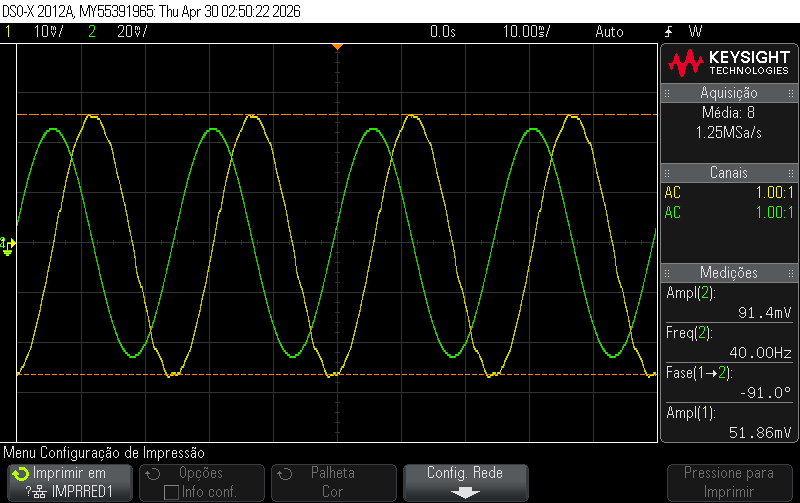
\includegraphics[width=0.7\linewidth]{FIGURAS/40Hz.png}
	\label{fig:osc_40hz}
\end{figure}

\begin{figure}[H]
	\centering
	\caption{Resposta no pico de ressonância (480 Hz).}
	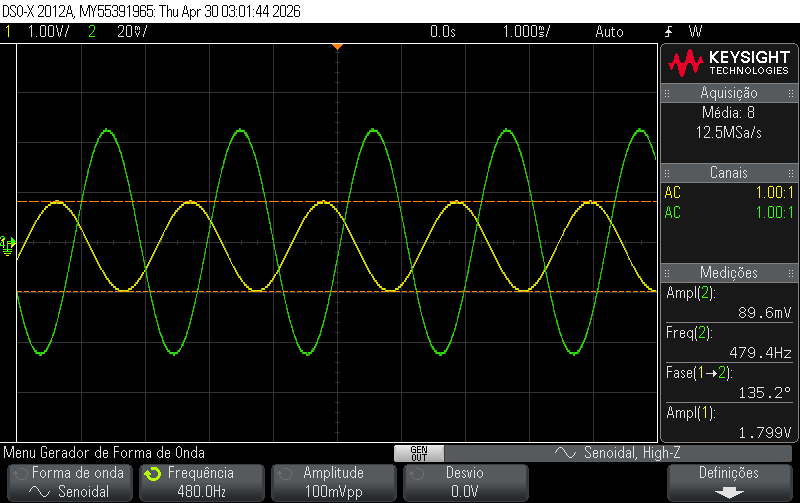
\includegraphics[width=0.7\linewidth]{FIGURAS/480Hz.png}
	\label{fig:osc_480hz}
\end{figure}

\subsection{Comportamento em Alta Frequência}

\begin{figure}[H]
	\centering
	\caption{Resposta do filtro em 5500 Hz.}
	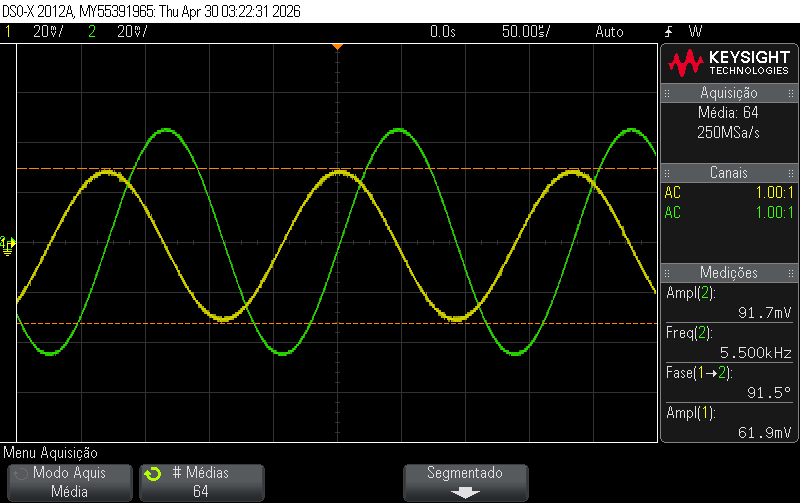
\includegraphics[width=0.7\linewidth]{FIGURAS/5500Hz.png}
	\label{fig:osc_5500hz}
\end{figure}

\begin{figure}[H]
	\centering
	\caption{Atenuação em alta frequência (11 kHz).}
	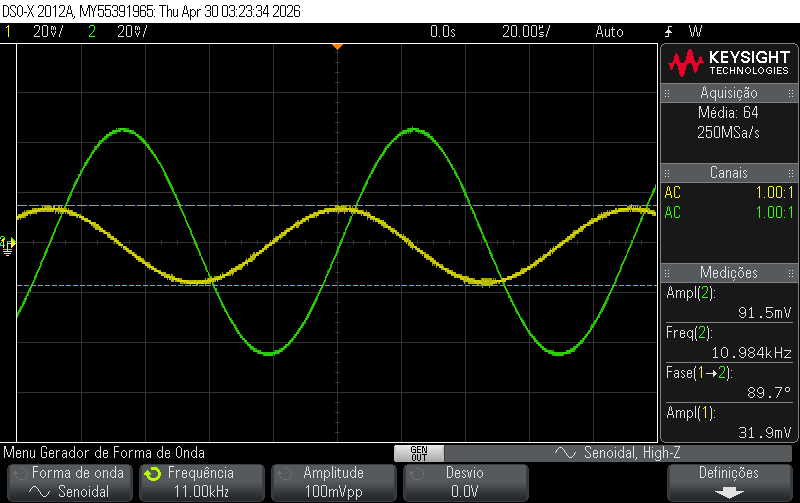
\includegraphics[width=0.7\linewidth]{FIGURAS/11kHz.png}
	\label{fig:osc_11khz}
\end{figure}

\section{Análise de Fontes de Erro}

As discrepâncias observadas entre o modelo matemático e os dados de bancada podem ser atribuídas aos seguintes fatores:

\begin{enumerate}
	\item \textbf{Tolerância dos Capacitores}: Capacitores cerâmicos ou de poliéster comumente possuem tolerâncias de $10\%$ a $20\%$. Como a frequência central $f_0$ e o ganho dependem de $C^2$ e $C$ respectivamente, este é o fator de maior impacto;
	
	\item \textbf{Produto Ganho-Banda (GBW)}: O amplificador operacional real possui ganho finito que decai com a frequência. Para ganhos elevados (próximos a 50 v/v), o limite do AmpOp pode achatar o pico do filtro;
	
	\item \textbf{Resistências Parasitas}: Contatos na \textit{protoboard} e a resistência interna do gerador de sinais podem alterar levemente a impedância de entrada vista pelo circuito;
	
	\item \textbf{Ruído de Medição}: Em frequências muito baixas ou muito altas, a amplitude do sinal de saída torna-se pequena, dificultando a medição precisa da fase pelo osciloscópio devido ao ruído de fundo.
\end{enumerate}

Apesar dos desvios, o comportamento global do circuito validou a topologia MFB, apresentando a característica de passa-faixa conforme previsto.